\documentclass[12pt,a4paper]{article}
\usepackage[utf8]{inputenc}
\usepackage[vietnamese]{babel}
\usepackage{graphicx}
\usepackage{float}
\usepackage{geometry}
\geometry{a4paper, margin=2.5cm}
\usepackage{hyperref}
\usepackage{xcolor}
\usepackage{fancyhdr}
\usepackage{titlesec}
\usepackage{booktabs}
\usepackage{listings}
\usepackage{array}

\hypersetup{
    colorlinks=true,
    linkcolor=blue,
    filecolor=magenta,      
    urlcolor=cyan,
    pdftitle={Bao cao Bai tap 1 - Quan ly tẹp va thu muc},
    pdfpagemode=FullScreen,
}

% Cấu hình header & footer
\pagestyle{fancy}
\fancyhf{}
\rhead{Hành trình Kỹ năng số}
\lhead{Bài tập Thực hành 1}
\rfoot{Trang \thepage}

% Định dạng tiêu đề mục
\titleformat{\section}{\normalfont\Large\bfseries\color{blue!80!black}}{\thesection}{1em}{}
\titleformat{\subsection}{\normalfont\large\bfseries\color{blue!60!black}}{\thesubsection}{1em}{}

\begin{document}

% --- TRANG BÌA ---
\begin{titlepage}
    \centering
    \vspace*{1cm}
    
    {\large \bfseries TRƯỜNG ĐẠI HỌC CÔNG NGHỆ - ĐHQGHN} \\[0.2cm]
    {\large \bfseries KHOA CÔNG NGHỆ THÔNG TIN} \\[1.5cm]
    
    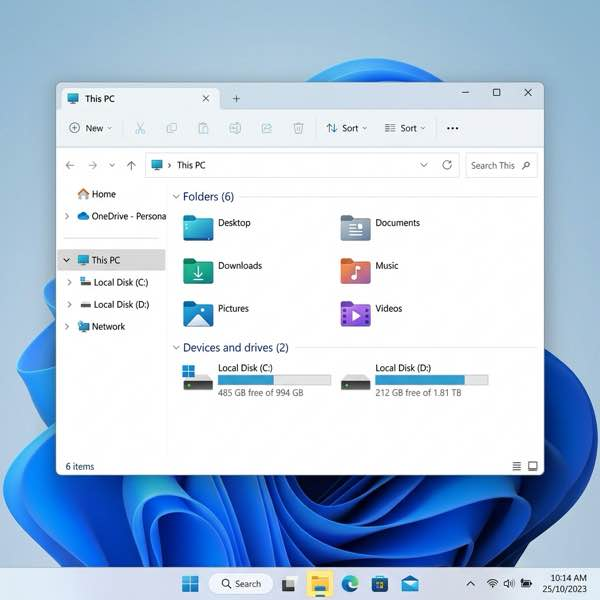
\includegraphics[width=0.3\textwidth]{images/step01.jpg} \\[1.5cm] % Sử dụng tạm ảnh đầu tiên làm ảnh đại diện bìa
    
    {\Large \bfseries BÁO CÁO BÀI TỰ THỰC HÀNH CÁ NHÂN} \\[0.5cm]
    {\Huge \bfseries BÀI TẬP 1: QUẢN LÝ TỆP TIN \& THƯ MỤC TRÊN HỆ ĐIỀU HÀNH} \\[1.5cm]
    
    \textbf{Môn học:} Nhập môn Công nghệ số và Ứng dụng Trí tuệ nhân tạo \\
    \textbf{Chủ đề:} Thao tác cơ bản và Nâng cao trên Windows 11 \\[2cm]
    
    \begin{flushleft}
        \large
        \textbf{Sinh viên thực hiện:} Nguyễn Bảo Đăng \\
        \textbf{Mã số sinh viên:} 25020115 \\
    \end{flushleft}
    
    \vfill
    {\large Năm 2026}
\end{titlepage}

\newpage
\tableofcontents
\newpage

% --- NỘI DUNG CHÍNH ---

\section{Giới thiệu và Mục tiêu bài thực hành}
Quản lý tệp tin và thư mục là một trong những kỹ năng số cốt lõi đối với bất kỳ người sử dụng máy tính nào, đặc biệt là các kỹ sư phần mềm tương lai. Việc lưu trữ dữ liệu một cách khoa học giúp tối ưu hóa không gian lưu trữ, tăng tốc độ truy tìm thông tin và nâng cao hiệu suất làm việc.

\subsection{Mục tiêu của bài thực hành}
\begin{itemize}
    \item Làm quen với giao diện của hệ điều hành Windows 11 và công cụ quản lý tập tin chuyên nghiệp \textbf{File Explorer}.
    \item Thực hiện thành thạo việc tạo lập, đặt tên và phân cấp hệ thống thư mục theo nguyên tắc khoa học.
    \item Nắm vững các thao tác thao tác cơ bản và nâng cao với tệp tin (Tạo mới, đổi tên, sao chép, di chuyển, xóa tạm thời, xóa vĩnh viễn và khôi phục).
    \item Phân biệt rõ sự khác nhau về bản chất giữa các thao tác sao chép (Copy) vs. di chuyển (Cut), và xóa tạm thời (Delete) vs. xóa vĩnh viễn (Shift+Delete).
\end{itemize}

\subsection{Yêu cầu hệ thống sử dụng}
\begin{itemize}
    \item Hệ điều hành: Microsoft Windows 11 Home / Pro.
    \item Công cụ: Windows File Explorer tích hợp sẵn.
\end{itemize}

\newpage
\section{Nhật ký thực hiện chi tiết từng bước}
Dưới đây là nhật ký chi tiết quá trình thực hiện bài tập thực hành quản lý tệp và thư mục trên máy tính cá nhân.

\subsection{Bước 1 \& 2: Khởi động công cụ File Explorer và chuẩn bị thư mục làm việc}
Để bắt đầu thực hành, chúng ta tiến hành khởi động File Explorer. Có hai cách thông dụng:
\begin{enumerate}
    \item Click vào biểu tượng thư mục màu vàng trên thanh Taskbar.
    \item Nhấn tổ hợp phím tắt \texttt{Windows + E}.
\end{enumerate}
Sau khi File Explorer xuất hiện, nhấn chọn thư mục \textbf{Documents} ở thanh điều hướng bên trái để chọn làm không gian làm việc chính.

\begin{figure}[H]
    \centering
    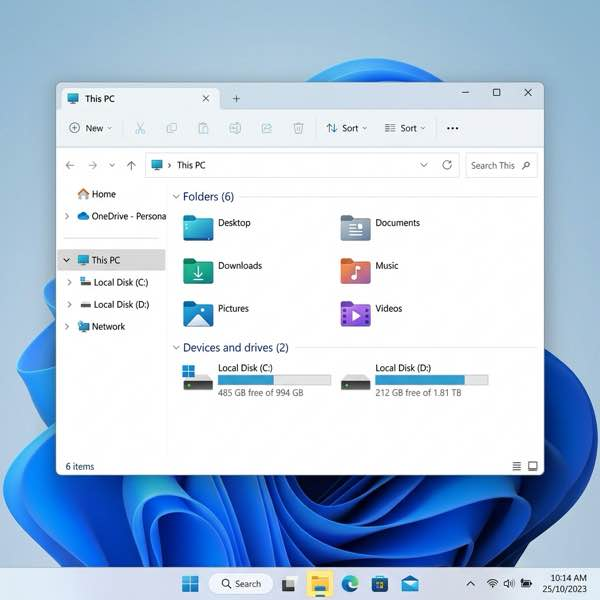
\includegraphics[width=0.9\textwidth]{images/step01.jpg}
    \caption{Giao diện File Explorer khi bắt đầu làm việc trong Documents}
    \label{fig:step01}
\end{figure}

\subsection{Bước 3: Tạo thư mục thực hành cá nhân}
Click chuột phải vào vùng trống trong thư mục \textbf{Documents}, rê chuột đến tùy chọn \textbf{New} và chọn \textbf{Folder} trên menu ngữ cảnh xuất hiện để tạo một thư mục mới.

\begin{figure}[H]
    \centering
    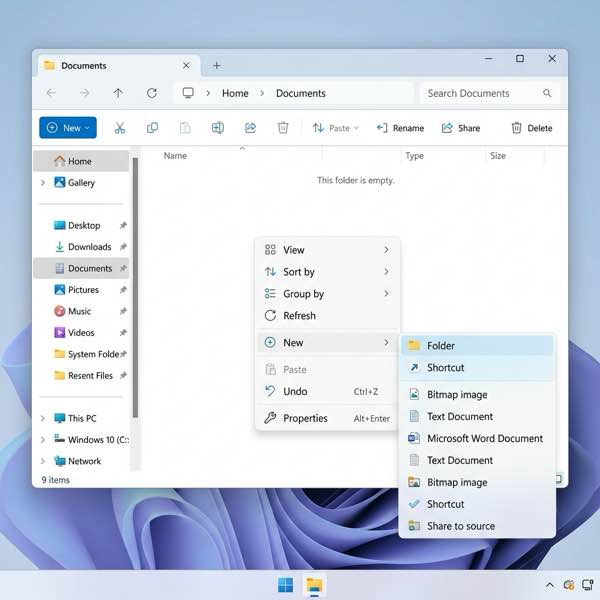
\includegraphics[width=0.9\textwidth]{images/step02.jpg}
    \caption{Menu ngữ cảnh Windows 11 khi tạo thư mục mới}
    \label{fig:step02}
\end{figure}

\subsection{Bước 4: Đổi tên thư mục thực hành}
Tại thư mục mới vừa tạo, ô nhập tên sẽ được bôi xanh để người dùng đặt tên. Tiến hành đặt tên thư mục theo cấu trúc \texttt{ThucHanh\_NguyenVanA} (Không dấu, có ký tự gạch dưới để tránh khoảng trắng gây lỗi khi xử lý đường dẫn) và nhấn \texttt{Enter}.

\begin{figure}[H]
    \centering
    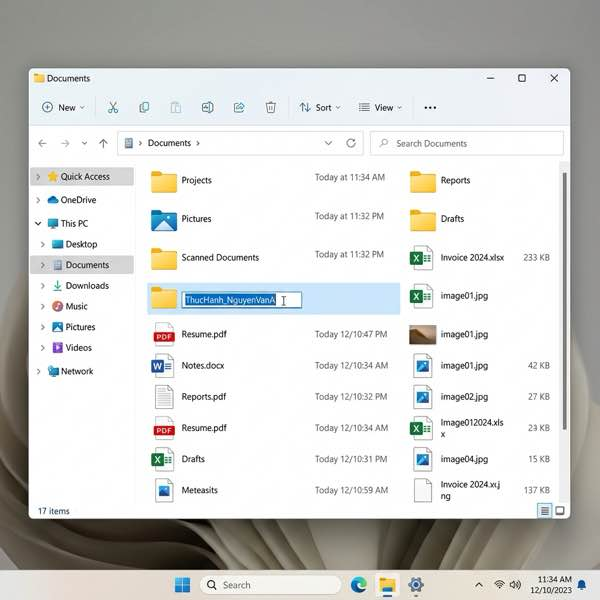
\includegraphics[width=0.9\textwidth]{images/step03.jpg}
    \caption{Thư mục thực hành \texttt{ThucHanh\_NguyenVanA} được tạo thành công}
    \label{fig:step03}
\end{figure}

\subsection{Bước 5: Tạo tệp tin văn bản mới}
Truy cập vào bên trong thư mục \texttt{ThucHanh\_NguyenVanA} vừa tạo bằng cách double-click chuột. Click chuột phải chọn \textbf{New} $\rightarrow$ \textbf{Text Document} để tạo một file văn bản thô (raw text file).

\begin{figure}[H]
    \centering
    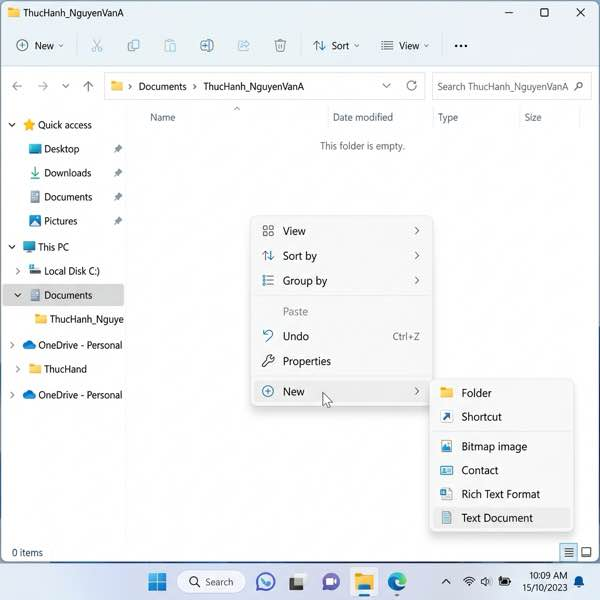
\includegraphics[width=0.9\textwidth]{images/step04.jpg}
    \caption{Tạo tệp tin văn bản mới trong thư mục thực hành}
    \label{fig:step04}
\end{figure}

\subsection{Bước 6: Đổi tên tệp tin văn bản}
Nhấp chuột phải vào tệp tin vừa tạo, chọn biểu tượng \textbf{Rename} (hoặc nhấn phím \texttt{F2} sau khi click chọn file) và nhập tên mới là \texttt{GhiChuQuanTrong.txt}, nhấn \texttt{Enter}.

\begin{figure}[H]
    \centering
    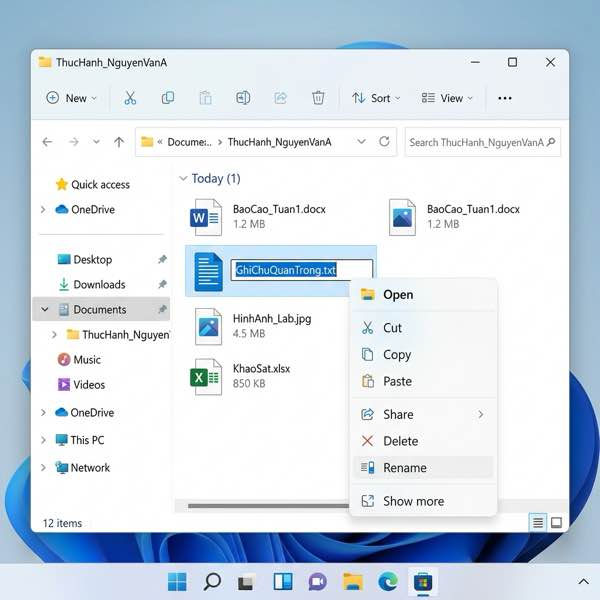
\includegraphics[width=0.9\textwidth]{images/step05.jpg}
    \caption{Đổi tên tệp văn bản thành \texttt{GhiChuQuanTrong.txt}}
    \label{fig:step05}
\end{figure}

\subsection{Bước 7: Tạo thư mục con phân cấp}
Tương tự như bước 3, tiến hành tạo một thư mục con bên trong thư mục \texttt{ThucHanh\_NguyenVanA} và đặt tên là \texttt{TaiLieu}. Thư mục này dùng để chứa các tài liệu cần phân loại.

\begin{figure}[H]
    \centering
    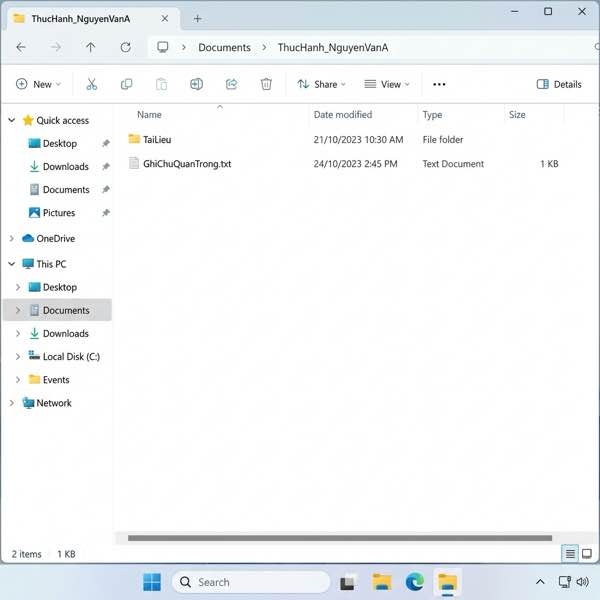
\includegraphics[width=0.9\textwidth]{images/step06.jpg}
    \caption{Cấu trúc thư mục gốc gồm thư mục \texttt{TaiLieu} và file \texttt{GhiChuQuanTrong.txt}}
    \label{fig:step06}
\end{figure}

\subsection{Bước 8: Sao chép tệp tin (Copy)}
Chọn tệp \texttt{GhiChuQuanTrong.txt}, nhấn tổ hợp phím \texttt{Ctrl + C} (hoặc click chuột phải và chọn biểu tượng \textbf{Copy}) để đưa tệp tin này vào bộ nhớ tạm thời của máy tính (Clipboard).

\begin{figure}[H]
    \centering
    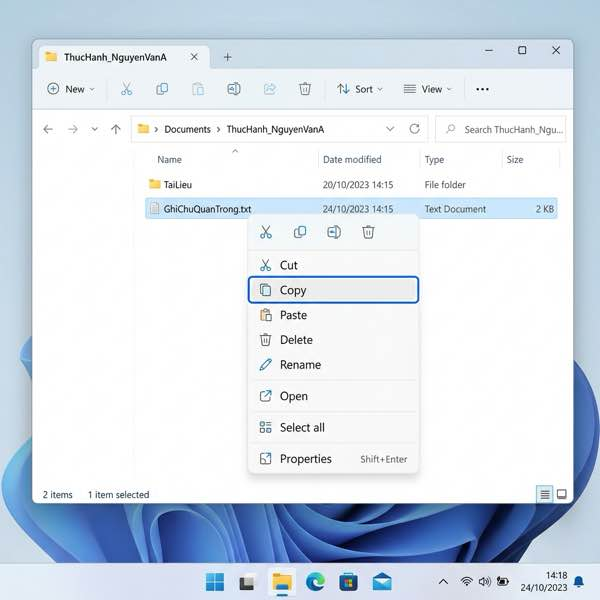
\includegraphics[width=0.9\textwidth]{images/step07.jpg}
    \caption{Thực hiện lệnh Copy trên tệp tin gốc}
    \label{fig:step07}
\end{figure}

\subsection{Bước 9: Dán tệp tin vào thư mục con (Paste)}
Mở thư mục con \texttt{TaiLieu} vừa tạo ở Bước 7. Nhấn tổ hợp phím \texttt{Ctrl + V} (hoặc click chuột phải vào vùng trống chọn biểu tượng \textbf{Paste}). Tệp tin đã được sao chép thành công vào thư mục con. Lúc này tệp tồn tại độc lập ở cả thư mục cha và thư mục con.

\begin{figure}[H]
    \centering
    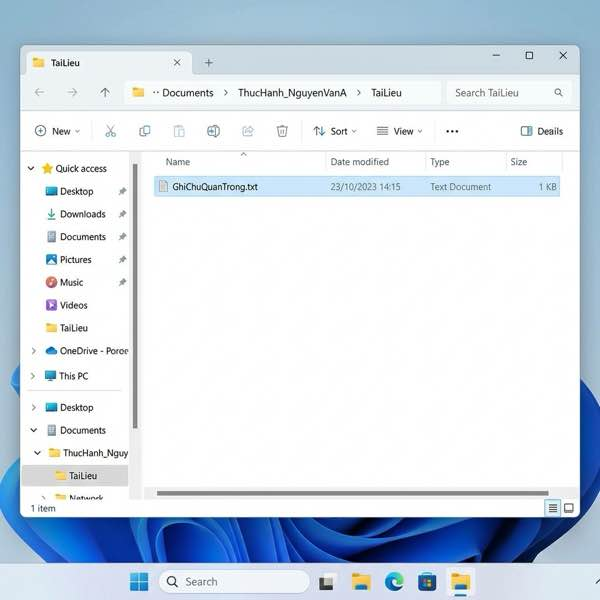
\includegraphics[width=0.9\textwidth]{images/step08.jpg}
    \caption{Dán tệp tin vào bên trong thư mục \texttt{TaiLieu}}
    \label{fig:step08}
\end{figure}

\subsection{Bước 10: Thực hành di chuyển tệp tin (Cut \& Paste)}
Tiến hành tạo một tệp tin khác có tên là \texttt{DiChuyen.txt} tại thư mục cha. Nhấp chọn tệp tin, nhấn tổ hợp phím \texttt{Ctrl + X} (hoặc chuột phải chọn \textbf{Cut}). Tệp tin sẽ có trạng thái mờ đi. Truy cập thư mục \texttt{TaiLieu} và nhấn \texttt{Ctrl + V}. Tệp tin sẽ chuyển hẳn vào thư mục con và không còn ở thư mục gốc.

\begin{figure}[H]
    \centering
    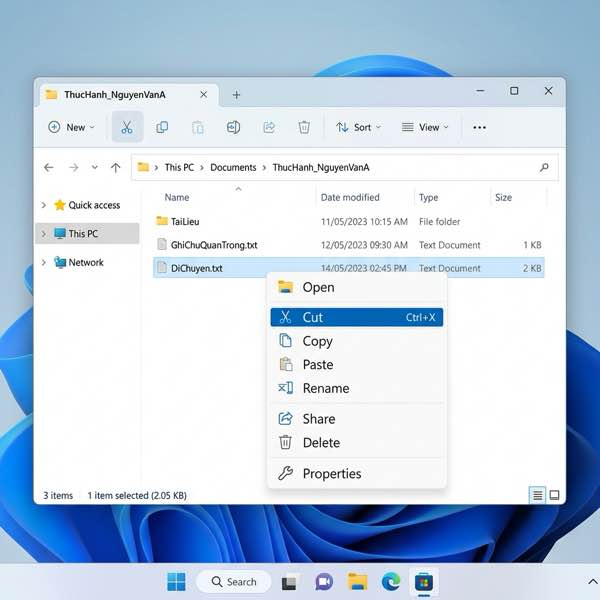
\includegraphics[width=0.9\textwidth]{images/step09.jpg}
    \caption{Thao tác Cắt (Cut) tệp tin \texttt{DiChuyen.txt} tại thư mục cha}
    \label{fig:step09}
\end{figure}

\subsection{Bước 11: Xóa tệp tin tạm thời vào Thùng rác (Delete)}
Truy cập thư mục con \texttt{TaiLieu}. Click chuột phải vào tệp \texttt{GhiChuQuanTrong.txt} mới được copy vào đây ở bước 9, chọn biểu tượng thùng rác hoặc nhấn phím \texttt{Delete} trên bàn phím. Tệp tin biến mất khỏi thư mục và được lưu trữ tạm trong Recycle Bin.

\begin{figure}[H]
    \centering
    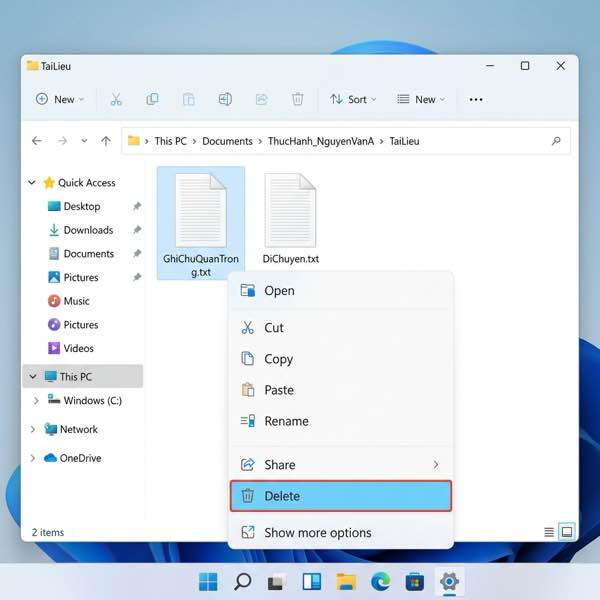
\includegraphics[width=0.9\textwidth]{images/step10.jpg}
    \caption{Xóa tệp tin \texttt{GhiChuQuanTrong.txt} vào Thùng rác}
    \label{fig:step10}
\end{figure}

\subsection{Bước 12: Xóa vĩnh viễn tệp tin (Shift + Delete)}
Chọn tệp tin \texttt{DiChuyen.txt} trong thư mục \texttt{TaiLieu}. Nhấn tổ hợp phím \texttt{Shift + Delete} trên bàn phím. Một hộp thoại cảnh báo của Windows 11 sẽ hiện lên để yêu cầu người dùng xác nhận việc xóa vĩnh viễn tệp tin này khỏi máy tính mà không qua Thùng rác. Nhấn \textbf{Yes}.

\begin{figure}[H]
    \centering
    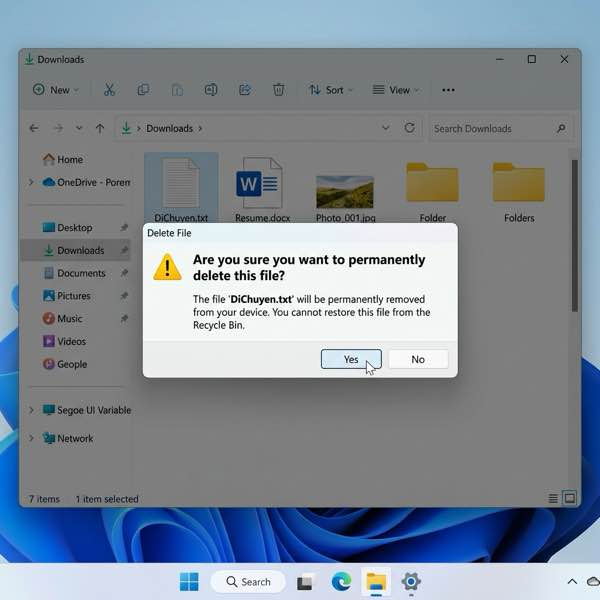
\includegraphics[width=0.8\textwidth]{images/step11.jpg}
    \caption{Hộp thoại cảnh báo xóa vĩnh viễn tệp tin của Windows 11}
    \label{fig:step11}
\end{figure}

\subsection{Bước 13: Khôi phục tệp tin đã xóa khỏi Thùng rác (Restore)}
Quay trở lại màn hình Desktop của Windows 11 và nhấp đúp chuột để mở \textbf{Recycle Bin} (Thùng rác). Tìm đến tệp tin \texttt{GhiChuQuanTrong.txt} đã xóa ở Bước 11. Nhấp chuột phải vào tệp và chọn \textbf{Restore}. Tệp tin sẽ tự động biến mất khỏi Thùng rác và quay trở về đúng vị trí trước khi bị xóa (Thư mục con \texttt{TaiLieu}).

\begin{figure}[H]
    \centering
    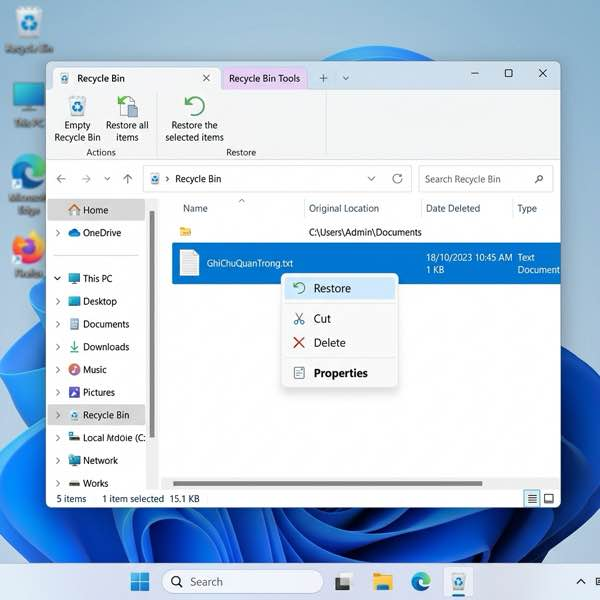
\includegraphics[width=0.9\textwidth]{images/step12.jpg}
    \caption{Menu ngữ cảnh khôi phục tệp tin trong Recycle Bin}
    \label{fig:step12}
\end{figure}

\newpage
\section{Bản chất kỹ thuật và Phân tích so sánh các thao tác}
Để hiểu sâu hơn về hệ thống tệp tin (File System) của hệ điều hành, dưới đây là phân tích chi tiết về mặt cơ chế giữa các nhóm thao tác.

\subsection{Sao chép (Copy) vs. Di chuyển (Cut)}
\begin{table}[H]
    \centering
    \caption{Bảng so sánh chi tiết thao tác Copy và Cut}
    \vspace{0.2cm}
    \begin{tabular}{|m{3.5cm}|m{5.5cm}|m{5.5cm}|}
        \hline
        \textbf{Tiêu chí so sánh} & \textbf{Sao chép (Copy \& Paste)} & \textbf{Di chuyển (Cut \& Paste)} \\
        \hline
        \textbf{Vị trí file gốc} & Vẫn được giữ nguyên ở thư mục ban đầu. & Bị xóa hoàn toàn khỏi thư mục ban đầu sau khi Paste thành công. \\
        \hline
        \textbf{Số lượng file tạo ra} & Tạo thêm một bản sao mới hoàn toàn độc lập. & Số lượng file giữ nguyên không đổi, chỉ thay đổi đường dẫn (path). \\
        \hline
        \textbf{Dung lượng đĩa} & Tiêu hao thêm dung lượng đĩa tương ứng kích thước file. & Không làm thay đổi dung lượng lưu trữ trên đĩa cứng. \\
        \hline
        \textbf{Tốc độ thực thi} & Tùy thuộc kích thước file (có quá trình đọc-ghi dữ liệu thực tế). & Cực nhanh đối với cùng một ổ đĩa (chỉ thay đổi bảng trỏ tệp tin MFT). \\
        \hline
    \end{tabular}
    \label{tab:copy_vs_cut}
\end{table}

\subsection{Xóa tạm thời (Delete) vs. Xóa vĩnh viễn (Shift + Delete)}
\begin{table}[H]
    \centering
    \caption{Bảng so sánh chi tiết thao tác Delete và Shift+Delete}
    \vspace{0.2cm}
    \begin{tabular}{|m{3.5cm}|m{5.5cm}|m{5.5cm}|}
        \hline
        \textbf{Tiêu chí so sánh} & \textbf{Xóa tạm thời (Delete)} & \textbf{Xóa vĩnh viễn (Shift + Delete)} \\
        \hline
        \textbf{Nơi lưu trữ file} & Chuyển vào Thùng rác (Recycle Bin). & Xóa khỏi bảng chỉ mục tệp tin, không vào Thùng rác. \\
        \hline
        \textbf{Giải phóng bộ nhớ} & Chưa giải phóng. Vẫn chiếm dung lượng lưu trữ của ổ cứng. & Giải phóng hoàn toàn dung lượng lưu trữ trên ổ cứng lập tức. \\
        \hline
        \textbf{Khả năng khôi phục} & Khôi phục cực kỳ đơn giản qua tính năng Restore trong Recycle Bin. & Rất khó khôi phục. Cần dùng các phần mềm khôi phục chuyên sâu (Recuva, EaseUS). \\
        \hline
        \textbf{Cảnh báo hệ thống} & Thường không cảnh báo hoặc chỉ thông báo nhẹ (tùy cài đặt). & Luôn có hộp thoại cảnh báo người dùng xác nhận. \\
        \hline
    \end{tabular}
    \label{tab:delete_vs_shiftdelete}
\end{table}

\newpage
\section{Kết luận và Bài học kinh nghiệm}
Thông qua bài thực hành cơ bản này, tôi đã rút ra được các kiến thức cốt lõi sau:
\begin{enumerate}
    \item \textbf{Cấu trúc thư mục khoa học:} Việc tổ chức thư mục nhiều cấp giúp quản lý một lượng lớn tài liệu học tập một cách trực quan, khoa học.
    \item \textbf{Quy tắc đặt tên (Naming Convention):} Nên đặt tên không dấu, viết hoa các từ đầu, hoặc dùng dấu gạch dưới (\_) làm phân tách. Tránh sử dụng các ký tự đặc biệt như \texttt{/, \textbackslash, *, ?, ", <, >, |} vì đây là các ký tự hệ thống Windows cấm sử dụng để tránh lỗi đường dẫn.
    \item \textbf{Phím tắt hệ thống:} Việc sử dụng thành thạo các phím tắt (\texttt{Ctrl+C}, \texttt{Ctrl+X}, \texttt{Ctrl+V}, \texttt{Delete}, \texttt{Shift+Delete}, \texttt{F2}, \texttt{Windows+E}) giúp nâng cao tốc độ xử lý công việc văn phòng lên gấp nhiều lần.
    \item \textbf{An toàn dữ liệu:} Nhận thức rõ sự nguy hiểm của tổ hợp \texttt{Shift+Delete}. Chỉ nên sử dụng khi chắc chắn tệp tin đó không còn giá trị sử dụng.
\end{enumerate}

\end{document}
